\documentclass[sigconf]{sigplanconf}
  \usepackage{lipsum}
  \usepackage[sorting=nyt,backend=bibtex]{biblatex}
 \bibliography{thesisbiblio} 
  \usepackage{graphicx}
  \usepackage{float}
  
  \usepackage{algorithm}
  \usepackage{algpseudocode}
  
  \makeatletter
  \def\BState{\State\hskip-\ALG@thistlm}
  \usepackage{makecell}
  \usepackage[table]{xcolor,colortbl}
  %\renewcommand\theadalign{bc}
  \renewcommand\theadfont{\bfseries}	
  
  
   \title{Memory virtualization overhead mitigation using contiguous memory virtual machines}
\authorinfo{
	LastName1, FirstName1\\
	\texttt{first1.last1@xxxxx.com}
	\and
	LastName2, FirstName2\\
	\texttt{first2.last2@xxxxx.com}
	\and
	LastName2, FirstName2\\
	\texttt{first2.last2@xxxxx.com}
}
  
  
 
\begin{document}
   \maketitle  
  
  \begin{abstract}
 Virtual machines are playing an increasing role in server consolidation, security, and fault tolerance as computing systems migrate to shared resources in the cloud. Since the software stack accesses data using virtual addresses, fast address translation is crucial for efficient data-centric computation and for providing the benefits of virtualization to a wide range of applications. Unfortunately, the overhead of virtualizing memory is not universally low. This overhead comes from costly hypervisor interventions and from translation lookaside buffer (TLB) misses which require the hardware to perform a two dimensional page walk, which may require up to 24 memory references on x86-64 architecture, rather than a native one dimensional page walk which could incur a maximum of 4 memory references. In this work, we propose a new mechanism of address translation in virtualized systems which is based on contiguous-memory virtual machines, and we show that its overall overhead is theoretically equivalent to that in native environments. Our basic idea is to map virtual machine physical address space to contiguous machine memory which would eliminate the need for a second page table during address translation. We developed a simulator to replay virtual machine traces from several well known data centers so as to demonstrate the feasibility of allocating contiguous machine memory to virtual machines using existing placement algorithms. We then implemented our solutions in the Xen hypervisor for paravirtualised virtual machines by eliminating any uneccessary hypercalls taking into consideration the fact that the virtual machine has a contiguous block of machine memory.
  \end{abstract}
  
 Keywords: Virtualization, Virtual Memory, Translation Lookaside Buffer, Contiguous Memory.
    \section{Introduction}
   Virtualization forms the foundation of our cloud infrastructure. It provides benefits including security, isolation, consolidation and fault tolerance, and enables easier scalability of applications and higher system utilization by abstracting the underlying hardware resources.
   These benefits became achievable because various hardware and software advances have substantially reduced the cost of virtualization \cite{gandhi}. Despite hardware and software acceleration \cite{gandhi} the overhead of virtualizing memory can still be very high.
   One of the largest contributors to performance overhead in virtualized environments is memory virtualization. An application executing on a guest operating system (OS) uses guest virtual addresses (gVA) that need to be translated to host physical addresses (hPA). The guest OS executes in guest physical address (gPA) space. To fully virtualize memory therefore, two levels of address translation are used: gVA$\rightarrow$ gPA : guest virtual address to guest physical address translation via a per-process guest page table (gPT) and gPA$\rightarrow$hPA : guest physical address to host physical address translation via a per-VM host page table (hPT). There are two state-of-the-art techniques to virtualize memory which provide different tradeoffs. The first is nested paging \cite{gandhi19}, which is a hardware technique whereby the host OS uses the gPT and the hPT simultaneously in order to get the final gVA$\rightarrow$hPA translation. In case of a TLB miss, the hardware performs a long-latency two dimensional (2D)page walk which could require up to 24 memory accesses \cite{gandhi19} in x86-64 systems. The second technique is called shadow paging \cite{gandhi57}, which requires the virtual machine monitor(VMM)to build a shadow page table (sPT) for each VM. The shadow page table contains gVA$\rightarrow$hPA translations and in case of a TLB miss, the hardware performs a fast native one dimensional (1D) page walk. However, page table updates on context switches require the VMM to perform substantial work to keep the page tables consistent \cite{gandhi10}. 
   Table \ref{tab:tradeoffs} summarizes the trade-offs provided by both shadow and nested paging as compared to base native.
   
   
   \begin{table}[!h]
   	\centering
   	\scalebox{0.75}{
   		\begin{tabular}{  >{\bfseries}cccc }
   			
   			& \thead{Base  Native} & \thead{Nested Paging} & \thead{Shadow Paging}\\
   			\hline
   			TLB Hit &\makecell{fast} &\makecell{fast} &fast \\
   			\hline
   			\makecell{Max. memory access \\ on TLB miss} & 4 &24 & 4\\
   			\hline
   			\makecell{Page table updates} & \makecell{fast\\direct} &\makecell{fast\\direct} & \makecell{slow\\mediated\\by VMM}\\
   			\hline
   			\makecell{Hardware support}&\makecell{1D\\page walk} & \makecell{2D\\page walk}&\makecell{1D\\page walk}\\
   			\hline
   		\end{tabular}
   	}
   	\caption{Trade-offs provided by shadow and nested paging as compared to base native}
   	\label{tab:tradeoffs}
   \end{table}   
   From the table Nested and Shadow paging both present significant overhead due to memory accesses and page table updates respectively, when compared to base native. With current hardware and software, the overheads of virtualizing memory are hard to minimize because a VM exclusively uses one technique or the other.
   In this paper, we introduce a new method of address translation based on virtual machines with contiguous machine memory. Our mechanism of address translation eliminates the need for a host page table, thereby leading to near native address translation overheads. We developed a software simulator to replay VM traces from MS Azure, Bitbrains and CERIT Scientic Cloud and our simulation results showed that a high percentage of VMs in these data centers can be allocated contiguous machine memory upon creation using a contiguity-aware placement algorith. 
   
    The basic idea behind our address translation mechanism is to allocate contiguous physical memory to virtual machines and introduce a hardware feature to store the base address of the contiguous chunk of machine memory. That is, we try to map a VM's guest physical address space to a chunk of contiguous host physical addresses. With such a memory layout, a virtual address in a guest OS gets translated to a physical address via simple addition, as shown in the equation:\textbf{ hPA = base\_address + gPA}. This mechanism of address translation could somehow complement existing virtual memory architecture and enable VMs with contiguous machine memory to benefit from a fast customized virtual-to-physical address mapping. Our memory address translation mechanism is handled by the hypervisor and is implemented by VMs with compatible memory architectures.    
   Our memory address translation technique can be summarized as follows:
  \paragraph{ \textit{Virtual-to-physical address translation.} 
  	} Using our technique of technique of address translation, the hypervisor starts by allocating contiguous machine memory to VMs upon creation. VMs which do not obtain contiguous machine memory use default memory virtualization techniques supported by the hypervisor. The hypervisor stores the base address of the contiguous chunk of memory in a specialized register. On a TLB miss for a given virtual address, a guest page table walk is done to obtain the corresponding address in guest physical memory. The real/machine address or host physical address is then obtained by applying the formula: \textbf{ hPA = base\_address + gPA}. Figure \ref{fig:summary} illustrates this idea.
  	 	
  	\begin{figure}[!h]
  		\centering 
  		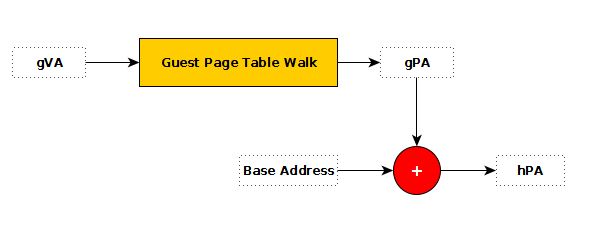
\includegraphics[scale=0.35]{mecanism.png}
  		\caption{x86\_64 native $VA \rightarrow PA$ translation}
  		\label{fig:summary}
  	\end{figure}
  	
  	Table \ref{tab:comparison} shows us a theoretical comparison of trade-offs provided by our translation model as compared to shadow and nested paging, and base native.
  	
  	\begin{table}[!h]
  		\centering
  		\scalebox{0.75}{
  			\begin{tabular}{  >{\bfseries}cccc|c }
  				
  				& \thead{Base \\ Native} & \thead{Nested \\ Paging} & \thead{Shadow \\ Paging}&\cellcolor{yellow!100}\thead{Our Solution}\\
  				\hline
  				TLB Hit &\makecell{fast} &\makecell{fast} &fast&\cellcolor{yellow!100} fast \\
  				\hline
  				\makecell{Max. memory access \\ on TLB miss} & 4 &24 & 4&\cellcolor{yellow!100}4\\
  				\hline
  				\makecell{Page table updates} & \makecell{fast\\direct} &\makecell{fast\\direct} & \makecell{slow\\mediated\\by VMM} &\cellcolor{yellow!100} \makecell{fast  direct}\\
  				\hline
  				\makecell{Hardware support}&\makecell{1D\\page walk} & \makecell{2D\\page walk}&\makecell{1D\\page walk}& \cellcolor{yellow!100} \makecell{1D page walk}\\
  				\hline
  			\end{tabular}
  		}
  		\caption{Trade-offs provided by our solution}
  		\label{tab:comparison}
  	\end{table}
  	
  	We notice that trade-offs provided using our solution are identical to base native. Our solution is clearly more efficient when compared to shadow or nested paging. 
  	
  	
  	
     \section{Memory virtualization overheads in X86-64 architecture}
     \subsubsection{Address translation in native systems}
     Processors based on the x86\_64 architecture use a radix tree of depth 4 for virtual to physical address translation in native systems \cite{dvmt}. We denote each layer in the tree as $L_i$, where $1 \leq i \leq 4$. Each node in the tree corresponds to a single physical memory frame which contains the physical frame numbers (memory addresses) of the child nodes. Leaf nodes hold the target frame number to which the source virtual address is mapped.     
     The address translation process is iterative and traverses a path from the root node to a leaf node. In each step, subsequent bit sets from the source virtual address are used to index the pages/nodes in the subsequent levels along the search path. Figure \ref{fig:1d} gives a simple illustration of this process. 
     
     \begin{figure}[!h]
     	\centering 
     	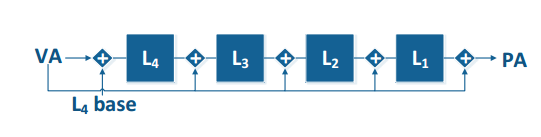
\includegraphics[scale=0.35]{1dtrans.png}
     	\caption{x86\_64 native $VA \rightarrow PA$ translation}{Source: \cite{dvmt}}
     	\label{fig:1d}
     \end{figure}
     
     \paragraph{Discussion.} The performance penalty of a valid page walk in x86\_64 native systems is \textbf{4 memory accesses}; Each memory access is done at each level of the page table structure/radix tree. This excessive overhead is mitigated using aggressive translation caches, which accelerate translation when workloads exhibit locality in virtual address space. 
     
     \subsubsection{Address translation in virtualized systems}
     Virtual machines require additional complexity when dealing with virtual address translation. Each process in a VM needs its own isolated virtual address space; Consequently, the system must provide translation from guest virtual addresses (gVA) to physical addresses on the host machine/host physical addresses (hPA). This translation is performed using a \textbf{nested page table}, which consists of a guest page table (gPT) in the VM and host page table (hPT) in the hypervisor. Each node in the guest radix tree points to a node in the next level using a guest physical frame number (which is still a host virtual address), and thus each transition between subsequent levels in the guest radix tree incures a full $gPA \rightarrow hPA$ using the hPT. This is referred to as a \textbf{two-dimensional (2D) page walk}. Figure \ref{fig:1d} illustrates a 2D page walk in x86\_64 systems.
     
     \begin{figure}[!h]
     	\centering 
     	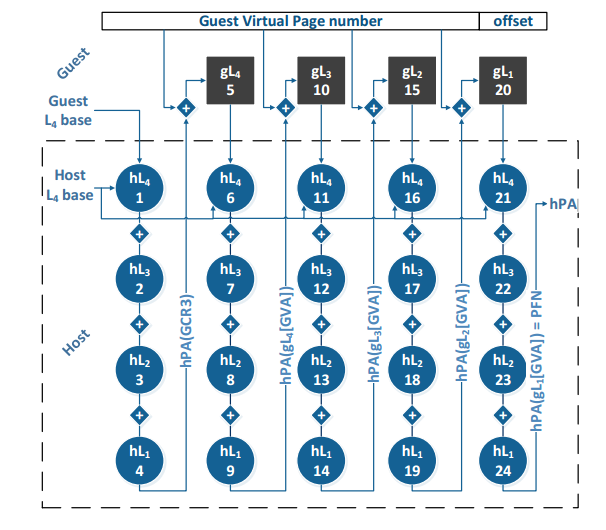
\includegraphics[scale=0.35]{2dtrans.png}
     	\caption{x86\_64 native $gVA \rightarrow hPA$ translation}{Source: \cite{dvmt}}
     	\label{fig:2d}
     \end{figure}
     
     \paragraph{Discussion.} Nested $gVA \rightarrow hPA$ translation dramatically increases the number of memory accesses to a total of \textbf{24 memory accesses}. This hugely affects the run time of VM workloads.
      \section{Benefits of address translation based on contiguous machine memory}
      The analysis of memory virtualization performance on x86 architecture indicates the costly nature of address translations in virtualized systems, which in turn leads to poor system performance in virtual machines. We could therefore argue that a more efficient mechanism of address translation which reduces the number of memory accesses incurred during translation could be of great benefit to VMs.
      
      VMs which are allocated contiguous machine memory throughout their execution and use our mechanism of address translation reduce translation overhead to near base native, as a result of the fact that we have a single page table traversal. Our simulation results show the feasibility of allocating contiguous machine memory to a huge percentage of VMs in data centers.
            
      We conclude that our address translation techniques based on contiguous memory virtual machines can go a very long way toward mitigatig address translation overheads in virtualized systems. The following section describes other related work that has been done towards 
       \section{RELATED WORK}
     \subsubsection{Flat Page Tables for VMs}
     Ahn et al.\cite{revisit} proposed replacing x86\_64's 4-level nested page table with a flat 1-level nested page table. This reduces the number of nested page table accesses from 4 to 1 and a 2D page walk from 24 to 8 memory references in total. While this is promising for the small virtual machines they studied, it may be less suited for big-memory workloads \cite{gandhi}.
     
     \subsubsection{Selective Hardware Software Paging (SHSP)}
     Past work - Selective Hardware Software Paging (SHSP) - showed that a hypervisor could dynamically switch an entire guest process between nested and shadow paging to achieve the best of either techniques \cite{gandhi101}. It monitored TLB misses and guest page faults to periodically consider switching to the best mode (less translation overhead). However, switching to shadow mode requires (re)building the entire shadow page table, which is expensive for multi-GB to TB workloads.
     
     \subsubsection{Multipage Mappings}
     Multipage Mapping approaches, such as sub-blocked TLBs \cite{gandhi96}, CoLT \cite{gandhi82} and Clustered TLBs \cite{gandhi81}, pack multiple PTEs into a single TLB entry. These designs leverage default OS memory allocators that either assign small blocks of contiguous physical pages to contiguous virtual pages (Sub-blocked TLBs and CoLT), or map small sets of contiguous virtual pages to clustered sets of physical pages (Clustered TLB). However, they pack only a small multiple of translations per entry, which limits their potential to reduce page walks for large workloads.
        \section{Architecture of our address translation mechanism}
       In this section, we give a more detailed explanation of our address translation technique.
       Figure \ref{fig:model_arch} depicts the overall flow of this mechanism. 
       
       \begin{figure}[!h]
       	\centering
       	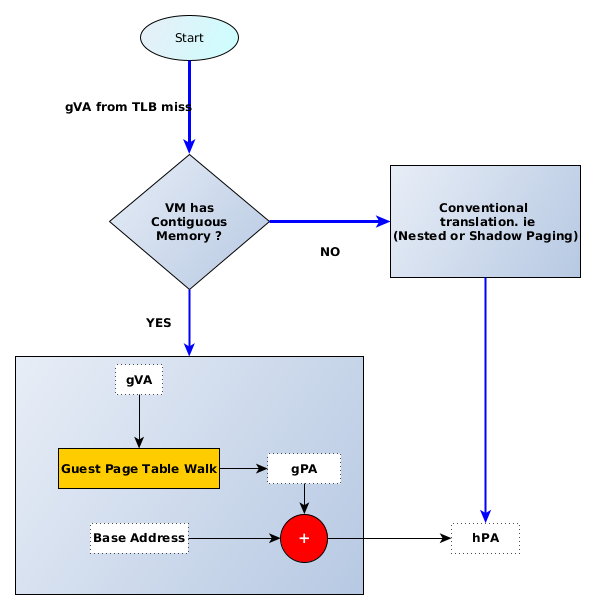
\includegraphics[scale=0.35]{meca_arch.png}
       	\caption{General architecture of our model}
       	\label{fig:model_arch}
       \end{figure}
       
       When a VM is being created, the hypervisor tries to allocate a contiguous chunk of machine memory to it. If it succeeds in doing this mapping, the hypervisor stores the \textbf{base address} of this contiguous chunk in a hardware register and maps the physical address space of the VM to this contiguous chunk as shown in figure 
       \ref{fig:cont_map}.
        
        \begin{figure}[!h]
        	\centering
        	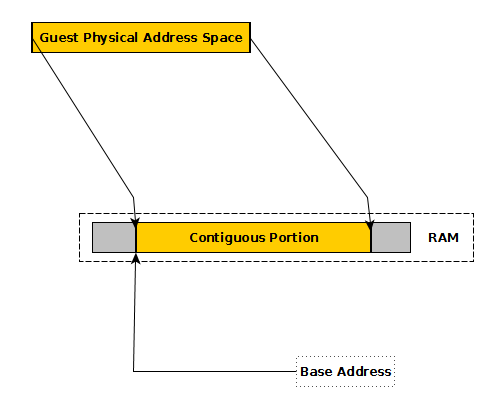
\includegraphics[scale=0.25]{map.png}
        	\caption{Contiguous memory mappingl}
        	\label{fig:cont_map}
        \end{figure}
       
       When a guest virtual address (gVA) is accessed, the TLB is checked first for the existence of a mapping. If the mapping is not found (TLB miss), the hypervisor starts by verifying if the guest physical address space is mapped to a contiguous piece of machine memory (RAM). If that is not the case, then the guest physical address space is not compatible with our address translation mechanism and the hypervisor uses conventional methods of address translation (nested or shadow paging) to perform the translation. In the ideal case, where the guest physical address space is mapped to a chunk of machine memory, the guest OS starts by performing a conventional guest page table walk (\textbf{4 memory references }) using the different bits of the gVA. The outcome of this page walk is the corresponding gPA. The VMM then reads the base address in the hardware register and adds the gPA to this base address in order to obtain the host physical address (hPA) or real address corresponding to the gVA. So we have a total of 4 memory references (same as base native) for a complete address translation. 
       
       \section{Reducing Fragmentation}
       The continuous creation and destruction of VMs with contiguous chunks of physical memory could prevent the allocation of contiguous machine memory at a certain point in time due to fragmentation. Moreover, the x86\_64 architecture fragments the guest physical memory of VMs for memory-mapped I/O\cite{gandhi}. We discuss a few ways to reduce memory fragmentation so as to increase the probability of contiguous memory allocation.
       
       \subsection{Memory Compaction}
       As physical pages are being allocated from a memory pool, the pool becomes fragmented. If some process requests a large piece of storage from the OS, the OS may not satisfy that request because there is no single contiguous chunk of memory that is large enough to satisfy the request, even though the total amount of free/unused storage in the pool is large enough. \textbf{Memory compaction} is simply the rearrangement of free and used pages so that the OS can satisfy the request.        
       Compaction is supported in many operating systems including Linux \cite{gandhi7}. Once the compaction daemon provides enough contiguous physical memory the VMM can allocate this to a VM upon creation. 
       
       
      \section{SIMULATION METHODOLOGY}
      In this section, we would discuss the inner workings of our simulation model and the significance of the different simulation results obtained.
            
      We recall that our address translation mechanism applies on VMs with \textbf{contiguous host physical memory}. That said, a study or \textbf{proof of concept} needs to be done so as to give us an idea of the percentage of VMs in real data centers with contiguous machine memory. In more formal terms, a proof of concept is simply a demonstration that proves the potential feasibility of an idea.
      
      For our feasibility study, we focused on aspects of real cloud workloads that have an impact on resource management. Thus, all of our datasets contain information about VM size (CPU cores and Memory size) and VM creation and deletion timestamps. We used VM traces from the following data centers: 
      \begin{itemize}
      	\item Microsoft Azure
      	\item CERIT Scientific Cloud
      	\item Bitbrains
      \end{itemize}
      We then developed a simulator to replay these traces using different \textbf{VM placement algorithms}.VM placement is the process of selecting the most suitable server in a large cloud data center to deploy newly-created VMs \cite{ieeeplacement}. Our simulation results provide an estimate of the percentage of VMs with contiguous memory during their lifetime.
      \subsubsection{Simulation Setup}
      To begin, let us introduce the simulation setup we used to estimate the percentage of contiguous memory VMs in datasets. For each dataset, we consider the resource requirement of each VM in terms of CPU cores and memory. We note that upon creation, each VM instance requires various resources such as number of virtual processors, memory and storage with different capacities. VM objects are created and destroyed according to their creation and destruction timestamps respectively. We take into consideration server generations and their resource capabilities for each dataset so as to provide more realistic results. We further assume that the resource capabilities of a datacenter are capable to host all the VMs in a given dataset.
      Our simulation algorithm simulates 2 major VM placement algorithms:
      \paragraph{Contiguity Aware Placement:}
      This algorithm prioritizes servers that can provide a VM with contiguous memory. That is, enough contiguous physical memory pages corresponding to the size of the VM's memory request. If no running server can satisfy the request, a new server is turned on and used. In case all servers are running and none can provide contiguous memory, the first server satisfying the resource request is chosen. The following pseudocode illustrates the contiguous aware placement algorithm.
      
      \begin{algorithm}  
      	\caption{Contiguity Aware VM Placement algorithm} 
      	\label{cont_aware}
      	\begin{algorithmic}[5]  
      		\Statex  
      		\Function{chooseContiguousServer}{vm,serverList}  
      		
      		\For{$i \gets 0 \textrm{ to } serverList.size$}  
      		\State tempServer = serverList.get (i);
      		\If{tempServer.hasContiguousMemory (VM) == true}  
      		\State \Return{tempServer}
      		\EndIf  
      		\EndFor  
      		\If{tempServer == NULL}
      		\State tempServer = possibleServers.get(0);
      		\EndIf
      		\State \Return{tempServer}  
      		\EndFunction  
      	\end{algorithmic}  
      \end{algorithm}
      
      \paragraph{Traditional Placement (Min/Max):}
      This algorithm simply takes into consideration resource availability in physical servers. The \textbf{Min} algorithm chooses the physical server with the least available resources among all the possible running servers that can host the VM instance. If no running server has enough available resources, a new server is turned on and used. The \textbf{Max} algorithm chooses the physical server with the most available resources among all the possible servers that can host the VM instance. The following pseudocode illustrates the Max and Min traditional placement algorithms.
      
      \begin{algorithm}  
      	\caption{Max Placement algorithm} 
      	\label{cont_aware}
      	\begin{algorithmic}[5]  
      		\Statex  
      		\Function{chooseMaxServer}{vm,serverList}  
      		\State availResources = vm.requiredResources;
      		\For{$i \gets 0 \textrm{ to } serverList.size$}  
      		\State tempServer = serverList.get (i);
      		\If{tempServer.availResources >= availResources}  
      		\State maxServer = tempServer;
      		\EndIf  
      		\EndFor  
      		\If{maxServer == NULL}
      		\State maxServer = new Server();
      		\EndIf
      		\State \Return{maxServer}  
      		\EndFunction  
      	\end{algorithmic}  
      \end{algorithm}
      
      \begin{algorithm}  
      	\caption{Min Placement algorithm} 
      	\label{cont_aware}
      	\begin{algorithmic}[5]  
      		\Statex  
      		\Function{chooseMinServer}{vm,serverList}  
      		\State availResources = vm.requiredResources;
      		\For{$i \gets 0 \textrm{ to } serverList.size$}  
      		\State tempServer = serverList.get (i);
      		\If{tempServer.availResources >= availResources}  
      		\State possibleServers.add (tempServer);
      		\EndIf  
      		\EndFor  
      		\State min = possibleServers.get(0).availResources;
      		\For{$i \gets 0 \textrm{ to } possibleServers.size$}  
      		\State tempServer = possibleServers.get (i);
      		\If{tempServer.availResources <= min}  
      		\State minServer = tempServer;
      		\EndIf  
      		\EndFor  
      		\If{minServer == NULL}
      		\State minServer = new Server();
      		\EndIf
      		\State \Return{minServer}  
      		\EndFunction  
      	\end{algorithmic}  
      \end{algorithm}
    
      
     
      
  \section{Evaluation}
  In this section, we would evaluate our idea as far as simulations are concerned. We would begin by explaining our evaluation methodology after which we would present the simulation results obtained. 
  
  \subsection{Evaluation Methodology}
  We carried out simulations on datasets from Microsoft Azure, CERIT Scientific Cloud, and Bitbrains. Each dataset comprises VM traces (.csv files) which contain information about the different VMs executed over a specific period of time in a data center. For each VM trace, the simulator uses one of the different placement algorithms described previously to choose a physical server object on which to host the VM object for its entire lifetime, which is determined by its creation and deletion timestamps. The simulator notes if the VM was allocated contiguous memory or not during its lifetime and at the end of the simulation, it calculates the percentage of VMs which were allocated contiguous memory during their lifetimes and the number of VMs and servers used for the simulation. The following section gives a brief description of the datasets we used for simulation.
  
  \subsubsection{Datasets} 
  As we mentioned above, our datasets come from 3 data centers: Microsoft Azure, CERIT Scientific Cloud, and Bitbrains. The characteristics of these datasets are as follows:
  \paragraph{Microsoft Azure dataset:} This dataset contains information about VMs running on Azure from November 16, 2016 to February 16, 2017. The trace information includes: identification numbers for each VM and the deployment and subscription to which it belongs; the VM role name; the VM size in terms of its maximum core, memory and disk allocations; and the minimum, average and maximum VM resource utilizations (reported every 5 minutes). Azure hosts both first-party and third-party workloads. First party workloads comprise internal VMs (research/development, infrastructure management etc) and third-party workloads comprise VMs created by external customers \cite{rescentral}. 
  Table \ref{tab:azure_servers} shows us the physical server composition we used in our simulation.
  \begin{center}
  	\begin{table}[!h]
  		\centering
  		\begin{tabular}{  l|l }
  			
  			\thead{Server Generation}&\thead{\%}\\
  			\hline 
  			Generatin 3&20\\
  			\hline
  			HPC&20\\
  			\hline
  			Generation 4&20\\
  			\hline
  			Generation 5&20\\
  			\hline
  			Generation 6&10\\
  			\hline
  			Godzilla&10\\
  		\end{tabular}
  		\caption{Physical server composition used for simulation}
  		\label{tab:azure_servers}
  	\end{table}
  \end{center}
  
  
  The following figures present an illustration of the virtual resource usage in the Microsoft Azure dataset.
  
  \begin{figure}[!h]
  	\centering
  	\begin{minipage}[t]{0.41\textwidth}
  		\centering
  		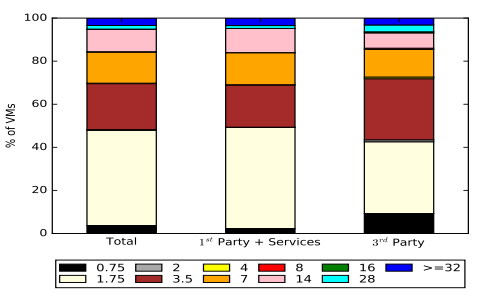
\includegraphics[scale=0.5]{azure_mem.png}
  		\caption{Amount of memory per VM in GB }
  		\label{azure)}
  	\end{minipage}
  	\hspace{2cm}
  	\begin{minipage}[t]{0.41\textwidth}
  		\centering
  		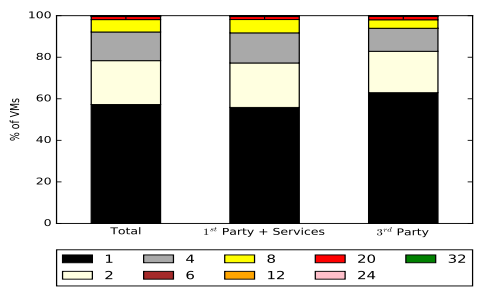
\includegraphics[scale=0.5]{azure_cores.png}
  		\caption{Number of virtual CPU cores per VM}
  		\label{fig:v4k}
  	\end{minipage}
  \end{figure}
  
  \newpage
  \paragraph{CERIT Scientific Cloud dataset:}
  This dataset represents the workload from 11,382 running VMs over a period of 1 year from CERIT Scientific Cloud \cite{cerit}. The physical infrastructure of CERIT-SC’s virtualized environment consists of six major clusters\footnote{ Groups of connected physical servers.} that vary heavily by means of their size and per-node parameters. Table \ref{tab:cerit} represents the cluster names and  charateristics:
  
  \begin{table}[!h]
  	\centering
  	\begin{tabular}{  l|l|l }
  		
  		\thead{Name}&\thead{RAM(GB)}&\thead{CPU(cores)}\\
  		\hline 
  		zapat&128&16\\
  		\hline
  		zebra&256&40\\
  		\hline
  		zigur&128&8\\
  		\hline
  		zegox&90&12\\
  		\hline
  		zefron&1000&40\\
  		\hline
  		zorg&512&40\\
  	\end{tabular}
  	\caption{CERIT-SC cluster characteristics}
  	\label{tab:cerit}
  \end{table}
  
  \paragraph{Bitbrains dataset:} This dataset comprises two groups of VM traces: The first group, fastStorage, consists of 1250 VMs connected to fast storage area network (SAN) devices and the second group, Rnd, consists of 500 VMs that are either connected to the fast SAN devices or the much slower Network Attached Storage (NAS) devices. The fastStorage trace includes a higher fraction of application servers while the Rnd trace includes mostly management machines which require lower storage as compared to the fastStorage VMs. VMs in the Bitbrains dataset use from 1 up to 32 CPU cores, but over 85\% of the VMs use at most 4 cores. On average, VMs in the Rnd dataset use slightly fewer cores. Most VMs in this dataset demand a maximum of 8GB of RAM but the VMs in the Rnd dataset demand slightly less memory than those in the fastStorage dataset, which request memory between 1 and 512GB \cite{bitbrains}.
  
  For simulation, we used the same server composition as that used for the Microsoft Azure dataset.
  
  
  \subsection{Experimental Setup}
  The simulations were carried out on a physical computer with the following characteristics:
  \begin{itemize}
  	\item 8 processors Intel (R) Core (TM), 2.60GHz
  	\item 8GB RAM memory 
  	\item Ubuntu 16.04 LTS Linux Kernel 4.15
  \end{itemize}
  
  
  \subsection{Simulation Results}
  In this section, we present the simulation results we obtained after replaying traces from the different datasets. The simulation results represent the percentage of VMs with contiguous memory using the VM placement algorithms we discussed above. NB: For each plot, the vertical axis is shifted so as to magnify the difference in percentages for the different placement algorithms.
  \paragraph{Microsoft Azure:} Figure \ref{fig:azure_res} shows the results obtained using the Microsoft Azure dataset.
  \begin{figure}[!h]
  	\centering
  	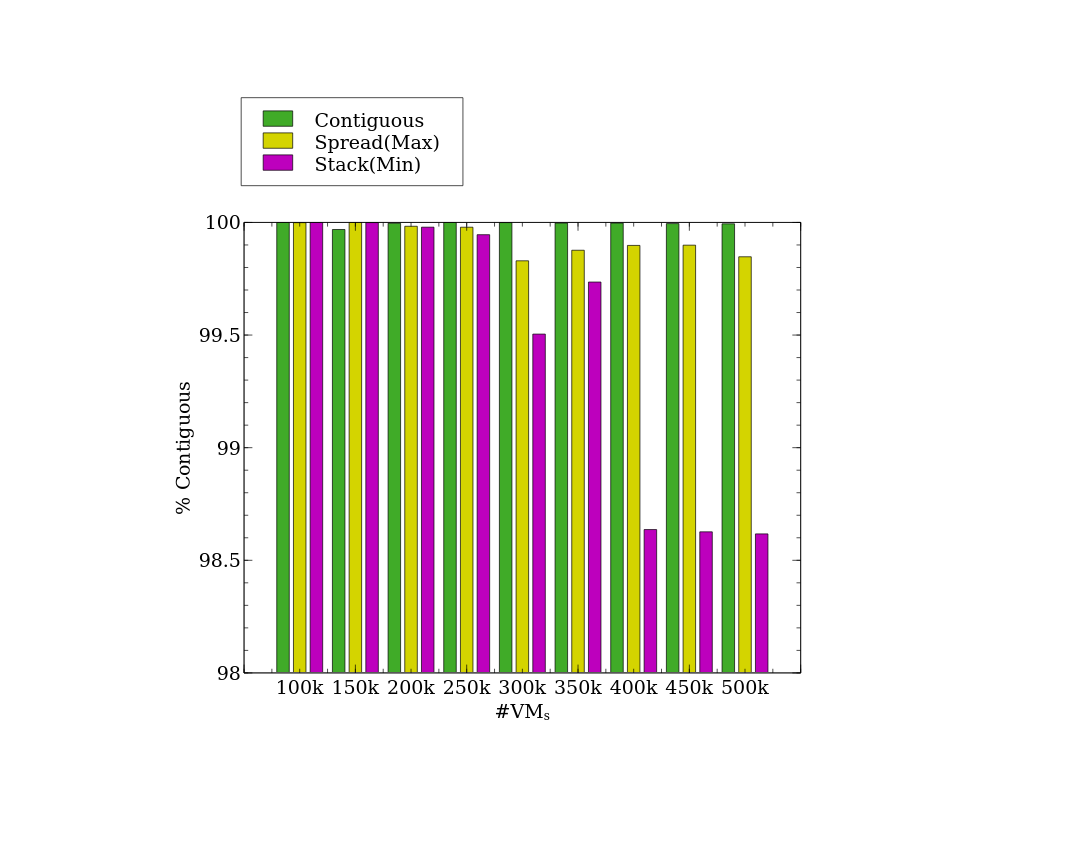
\includegraphics[scale=0.4]{azure-final.png}
  	\caption{Percentage of contiguous-memory VMs in the Microsoft Azure dataset}
  	\label{fig:azure_res}
  \end{figure}
  We have very high numbers of VMs with contiguous memory using the different placement algorithms. This is because the VM sizes are very small compared to server sizes. Nevertheless, this shows that a pretty large percentage of VMs in this datacenter could be given contiguous memory. 
  
  \paragraph{CERIT-SC:} 
  Figure \ref{fig:cerit_res} shows the results obtained using the CERIT-SC dataset.
  \begin{figure}[!h]
  	\centering
  	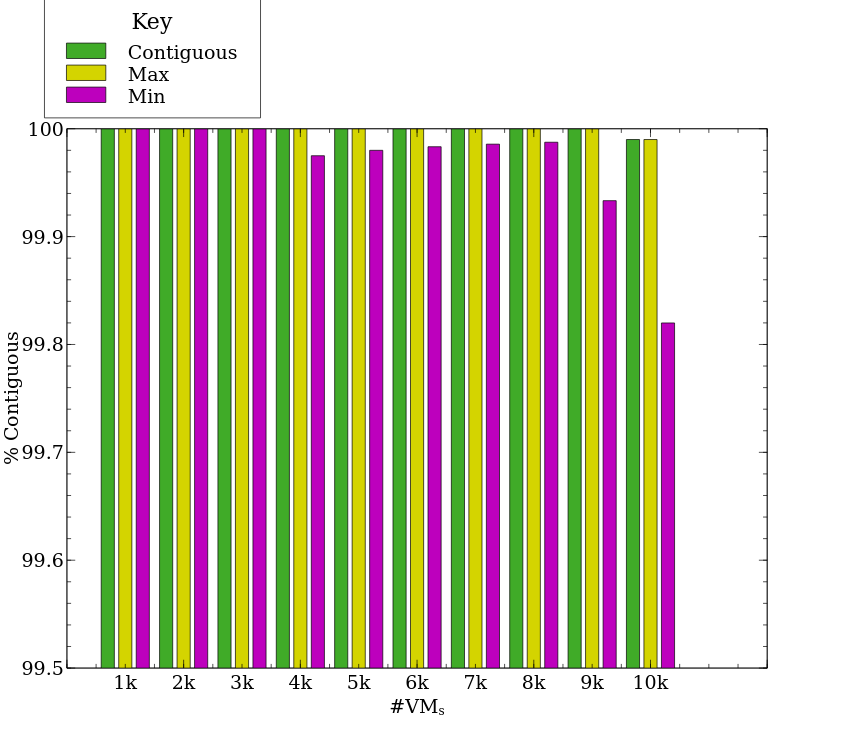
\includegraphics[scale=0.35]{cerit-final.png}
  	\caption{Percentage of contiguous-memory VMs in the CERIT-SC dataset}
  	\label{fig:cerit_res}
  \end{figure}
  
  \paragraph{Bitbrains:} 
  Figure \ref{fig:cerit_res} shows the results obtained using the Bitbrains dataset.
  \begin{figure}[!h]
  	\centering
  	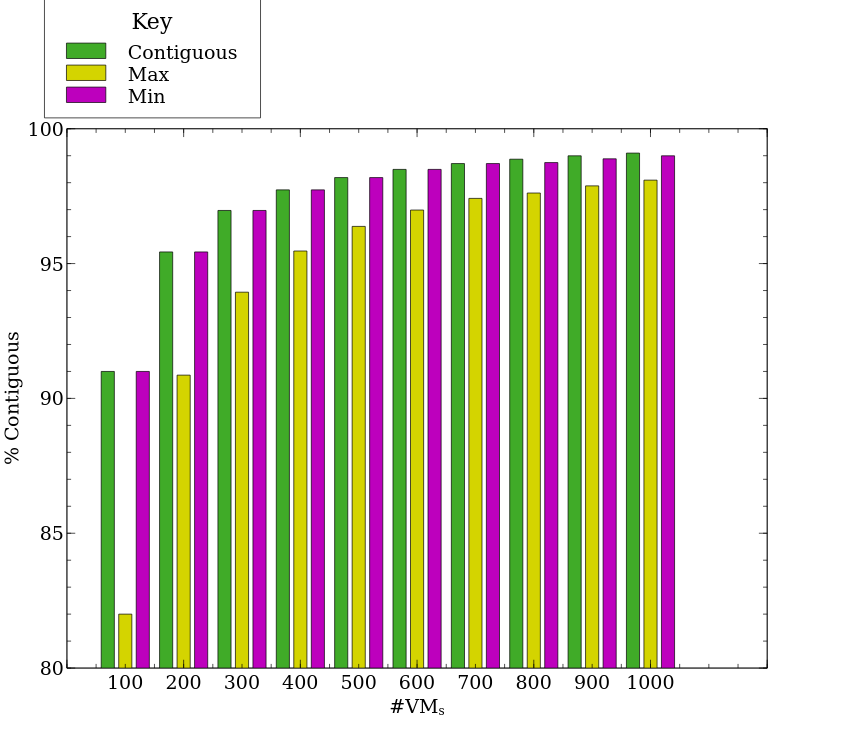
\includegraphics[scale=0.35]{bitbrains-fast.png}
  	\caption{Percentage of contiguous-memory VMs in the Bitbrains dataset (fastStorage)}
  	\label{fig:cerit_res}
  \end{figure}
  \newline
  We still have a high percentage of contiguous-memory VMs here for each placement algorithm. However, this percentage is lower in general when compared to the other datasets. This is because the VMs in the Bitbrains dataset have quite high resource demands compared to VMs in the other datasets. The contiguous aware placement algorithm, nevertheless, gives the highest percentage of contiguous memory to VMs.
  
  \paragraph{Consolidation Rate:} Here, we define the \textbf{consolidation rate} as the ratio of servers used to the total number of servers in the data center. It is important for a new placement algorithm to present a good consolidation rate when compared to existing placement methods. That is, the new placement algorithm should not increase the total number of servers used for a given dataset when compared to existing placement algorithms. Figure \ref{consolidation} illustrates the variation in consolidation rate for the MS Azure dataset.
  \begin{figure}[!h]
  	\centering
  	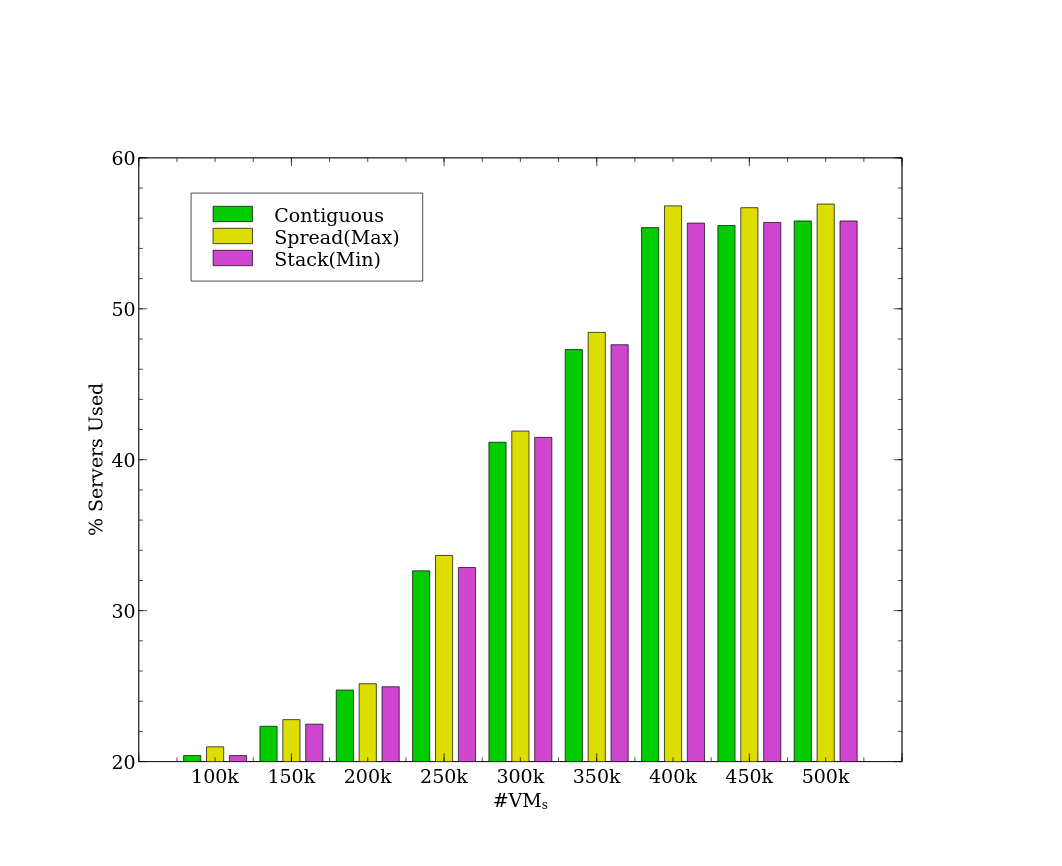
\includegraphics[scale=0.35]{servers.png}
  	\caption{Consolidation Rates for the different placement algorithms}
  	\label{consolidation}
  \end{figure}
  We observe that the consolidation rate is similar for the different placement algorithms which means our contiguity aware placement algorithm makes little changes to the consolidation rate when compared to traditional placement algorithms.
  \subsection{Analysis of Results}
  From the different results illustrated above, we observe that for each dataset we have a reasonably high percentage of contiguous memory VMs with the different VM placement algorithms. These high percentages are as a result of the fact that most VM sizes in data centers are small when compared to physical server sizes, as illustrated in most of the datasets. With a small degree of fragmentation on a physical server, there is therefore a high probability of allocating contiguous machine memory to a virtual machine. 
  
  \section{Hypervisor modification}
  
  \subsubsection{Contiguous Memory Allocation }
  This was the very first part of our hypervisor implementation and the importance of this should be obvious: our solution is based on contiguous memory VMs. In order to proceed, we must first understand what happens when a Xen VM is created.
  
  Xen uses a \textbf{configuration file} to create a VM. The configuration file contains information such as the amount of memory (in MB) to allocate to a VM, number of virtual CPUs, network related information etc. For the sake of simplicity, we would limit ourselves to memory related information. Xen uses the memory information in the configuration file to estimate the number of physical pages to be allocated to the VM. Recall, in x86 systems, a physical page is \textbf{4KB} in size. These pages are then allocated and mapped to the guest physical address space of the VM.
  
  \paragraph{How Xen allocates physical memory pages:}
  In Xen, the \textbf{Xen Heap} is in charge of allocating free pages to VMs on demand. The Xen Heap is a specialized data structure which contains all the addresses of free memory segments and pages in machine memory. By default, Xen allocates pages in batches of \textbf{4KB}, \textbf{2MB}, or \textbf{1GB}. For efficiency reasons, the Xen Heap does not allocate pages 4KB at a time. To allocate a batch of pages, Xen must calculate the \textbf{order} corresponding to the number of pages in the batch and pass this order to the Xen heap allocator. The relationship between the order and the number of pages is given below:
  \begin{center}
  	\textbf{ $2^{ order}$ = Number of 4KB pages}
  \end{center}
  This means a group of 4 contiguous pages has an order of 2, a group of 512 contiguous pages (2MB) has an order of 9 and a group 262,144 4KB contiguous pages (1GB) has an order of 18. A single 4KB page would have an order of 0. To allocate, for example, a 1GB chunk of memory pages, we need to pass the order 18 to the Xen heap allocator. In Xen, contiguous chunks of physical pages are referred to as \textbf{extents.} The maximum order of an extent Xen can handle is 20, which corresponds to an extent of 4GB. To understand how the Xen heap finds extents of different orders, it is important for us to master the structure of the Xen heap. 
  
  \paragraph{Structure of the Xen heap:} The Xen heap is tree-like in structure and the heap itself could be seen as the root of the tree. The heap consists of nodes and each node consists of zones. Each zone comprises a number of lists which contain the addresses of extents of a specific order. Each list is indexed by the order of the extents it contains. A list $L_i$ for example, would contain the addresses of free extents of order \textbf{i} within that zone. Figure \ref{fig:xenheap} illustrates this.
  
  \begin{figure}[!h]
  	\centering
  	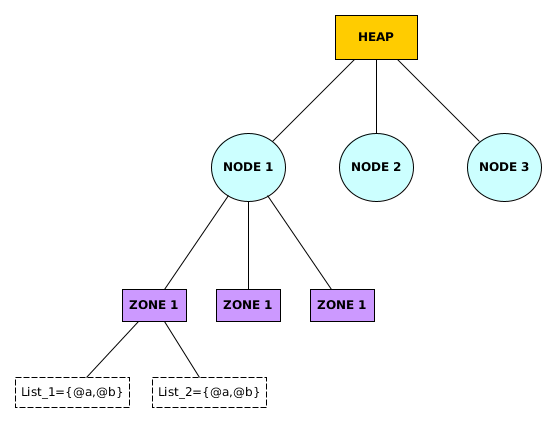
\includegraphics[scale=0.45]{xen_heap.png}
  	\caption{The Xen Heap Structure}
  	\label{fig:xenheap}
  \end{figure}
  \newpage
  As we can see, the Xen heap has a very elegant design but we have a little problem at the level of contiguity: the Xen heap does not necessarily allocate extents in a contiguous fashion. To solve this problem, we had to modify the heap allocator in such a way that it allocates all extents for Domain U guests in a contiguous fashion. NB: To know if a group of pages are contiguous, we calculate the \textbf{machine frame number (MFN)}\footnote{ A number that identifies a page/frame in RAM memory.} of each page and check if the MFNs of all the pages are consecutive. The following pseudocode gives a brief summary of the core modifications we made in the Xen heap allocator so as to achieve our goal.
  \newpage
  \begin{algorithm}  
  	\caption{Xen Heap Allocator} 
  	\label{cont_aware}
  	\begin{algorithmic}[5]  
  		\Statex  
  		\Function{alloc\_heap\_page}{order,node}  
  		\State next\_mfn = 0;
  		\State zone = zone\_hi;
  		\While {$zone>zone\_lo$}
  		\For{$i \gets order \textrm{ to } MAX\_ORDER$}  
  		\If{(!page\_list\_empty(heap(node,zone,i)))}  
  		\ForAll{(page in heap(node,zone,i))}
  		\If{page.mfn == next\_mfn}
  		\State next\_mfn+=page.size;
  		\State goto found;
  		\EndIf
  		\EndFor
  		\EndIf  
  		\EndFor
  		\State zone - -
  		\EndWhile
  		
  		\State found: ...
  		\EndFunction  
  	\end{algorithmic}  
  \end{algorithm}
  
  The Xen heap allocator is of course more complex than what is illustrated in the above code. Nevertheless, the above algorithm gives us an idea of how we force the Xen heap allocator to allocate pages in a contiguous fashion. In the case where it is impossible to allocate contiguous pages, the Xen heap allocator uses its default algorithm, and our translation mechanism cannot be applied. 
  
  \subsubsection{Address Translation}
  Domain U PV guests in Xen use \textbf{direct paging} for address translation \cite{xenorg}. Here the guest OS uses a \textbf{physical to machine (P2M)} mapping to map guest physical addresses to machine addresses. P2M mappings map guest physical addresses directly to machine addresses and as such the guest OS uses machine addresses directly when it writes its page tables. Our contiguous memory allocations make its very easy to build the P2M table in Domain U PV guests as all pages are contiguous. Furthermore, it becomes possible to eliminate unnecessary hypercalls in PV guests since they somehow have access to a specified range of contiguous machine memory.
  
  Applying our solution to Domain U HVM guests is quite complex because we need additional hardware (which is absent in the default architecture). As such, we can only evaluate our mechanism through simulation in the case of Xen HVMs. 
      
         
 \section{CONCLUSIONS}
 \lipsum[3]
 \section{ACKNOWLEDGEMENTS}
 \lipsum[3]
\printbibliography
\end{document}